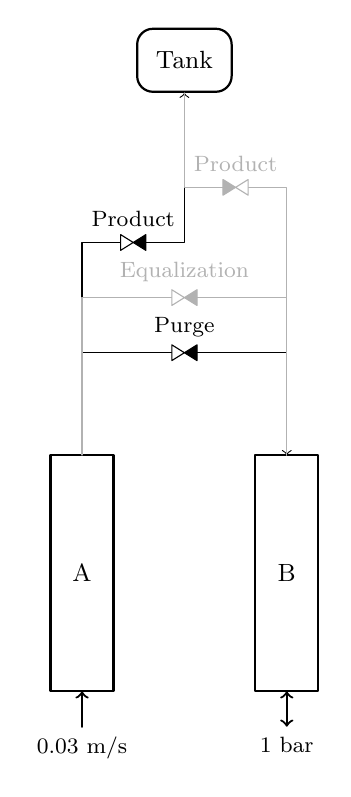
\begin{tikzpicture}[line cap=round, line join=round, font=\small]
  % Symbols: a valve, a check valve (filled towards its outlet), and a compressor, each with its outlet at +x.
  \tikzset{
    valve/.pic={\draw[fill=white] (-0.16,-0.1) -- (0.16,0.1) -- (0.16,-0.1) -- (-0.16,0.1) -- cycle;},
    check valve/.pic={\draw[fill=white] (-0.16,-0.1) -- (0,0) -- (-0.16,0.1) -- cycle;
                      \draw[fill] (0.16,-0.1) -- (0,0) -- (0.16,0.1) -- cycle;},
    compressor/.pic={\draw[fill=white] (0,0) circle (0.18); \draw (-0.09,-0.156) -- (0.18,0) -- (-0.09,0.156);}}
  \draw[thick] (-0.40,0) rectangle (0.40,3.00); \node at (0.00,1.50) {A};
  \draw[thick] (2.20,0) rectangle (3.00,3.00); \node at (2.60,1.50) {B};
  \node[draw, thick, rounded corners=0.2cm, minimum width=1.2cm, minimum height=0.8cm, anchor=south] at (1.30,7.60) {Tank};
  \draw[->] (0.00,3.00) -- (0.00,5.70) -- (1.30,5.70) -- (1.30,7.60);
  \pic[xscale=1] at (0.65,5.70) {check valve}; \node[above=0.08cm] at (0.65,5.70) {\footnotesize Product};
  \draw[->] (0.00,3.00) -- (0.00,4.30) -- (2.60,4.30) -- (2.60,3.00);
  \pic[xscale=1] at (1.30,4.30) {check valve}; \node[above=0.08cm] at (1.30,4.30) {\footnotesize Purge};
  \draw[gray!60] (0.00,3.00) -- (0.00,5.00) -- (2.60,5.00) -- (2.60,3.00);
  \pic[gray!60][xscale=1] at (1.30,5.00) {check valve}; \node[gray!60][above=0.08cm] at (1.30,5.00) {\footnotesize Equalization};
  \draw[gray!60] (2.60,3.00) -- (2.60,6.40) -- (1.30,6.40) -- (1.30,7.60);
  \pic[gray!60][xscale=-1] at (1.95,6.40) {check valve}; \node[gray!60][above=0.08cm] at (1.95,6.40) {\footnotesize Product};
  \draw[<-, thick] (0.00,0.00) -- (0.00,-0.45) node[below] {\footnotesize 0.03 m/s};
  \draw[<->, thick] (2.60,0.00) -- (2.60,-0.45) node[below] {\footnotesize 1 bar};
\end{tikzpicture}
